% EDC_Proton_Junction_Model.tex
% Companion F to Paper 3: Proton as 5D Junction — Variational Foundation
% Version 1.0 — 2026-01-19
% Build: XeLaTeX (Unicode)

\documentclass[11pt,a4paper]{article}

% ============================================================
%  PACKAGES
% ============================================================
\usepackage{fontspec}
\usepackage{amsmath,amssymb,amsthm}
\usepackage{mathtools}
\usepackage{physics}
\usepackage{geometry}

% FONTS (TeX Gyre Termes = Times-like with full OpenType support)
\IfFontExistsTF{TeX Gyre Termes}{%
  \setmainfont{TeX Gyre Termes}
  \setsansfont{TeX Gyre Heros}
}{%
  \setmainfont{Times New Roman}[Ligatures=TeX]
  \setsansfont{Helvetica}
}
\geometry{margin=2.5cm}
\usepackage{hyperref}
\hypersetup{
    colorlinks=true,
    linkcolor=blue,
    citecolor=blue,
    urlcolor=blue,
    pdfborder={0 0 0}
}
\usepackage{enumitem}
\usepackage{booktabs}
\usepackage{array}
\usepackage{xcolor}
\usepackage{tcolorbox}
\usepackage{tikz}
\usetikzlibrary{calc,angles,quotes,decorations.markings}
\usepackage{gensymb}

% ============================================================
%  EPISTEMIC TAG COMMANDS
% ============================================================
\definecolor{tagDer}{RGB}{0,128,0}      % Green - Derived
\definecolor{tagDc}{RGB}{0,0,200}       % Blue - Deduced/Constrained
\definecolor{tagCal}{RGB}{200,0,0}      % Red - Calibrated
\definecolor{tagP}{RGB}{128,0,128}      % Purple - Postulated
\definecolor{tagBL}{RGB}{128,128,128}   % Gray - Baseline
\definecolor{tagI}{RGB}{255,140,0}      % Orange - Identified
\definecolor{tagOpen}{RGB}{200,100,0}   % Dark orange - Open

\newcommand{\tagDer}{\textcolor{tagDer}{\textbf{[Der]}}}
\newcommand{\tagDc}{\textcolor{tagDc}{\textbf{[Dc]}}}
\newcommand{\tagCal}{\textcolor{tagCal}{\textbf{[Cal]}}}
\newcommand{\tagP}{\textcolor{tagP}{\textbf{[P]}}}
\newcommand{\tagBL}{\textcolor{tagBL}{\textbf{[BL]}}}
\newcommand{\tagI}{\textcolor{tagI}{\textbf{[I]}}}
\newcommand{\tagOpen}{\textcolor{tagOpen}{\textbf{[OPEN]}}}
\newcommand{\tagDef}{\textcolor{tagDc}{\textbf{[Def]}}}

% ============================================================
%  THEOREM ENVIRONMENTS
% ============================================================
\newtheorem{postulate}{Postulate}
\newtheorem{definition}{Definition}[section]
\newtheorem{theorem}{Theorem}[section]
\newtheorem{lemma}[theorem]{Lemma}
\newtheorem{corollary}[theorem]{Corollary}
\newtheorem{proposition}[theorem]{Proposition}
\newtheorem{remark}{Remark}[section]

% ============================================================
%  CUSTOM COMMANDS
% ============================================================
\newcommand{\re}{r_e}
\newcommand{\Ztwo}{\mathbb{Z}_2}
\newcommand{\Ztri}{\mathbb{Z}_3}
\newcommand{\Zthree}{\mathbb{Z}_3}
\newcommand{\Zsix}{\mathbb{Z}_6}
\newcommand{\Sthree}{S^3}
\newcommand{\Stwo}{S^2}
\newcommand{\Bthree}{B^3}
\newcommand{\Mfive}{\mathcal{M}_5}
\newcommand{\Bfour}{\mathcal{B}_4}
\newcommand{\tension}{\tau}  % string/flux-tube tension (E/L)

% ============================================================
%  TITLE
% ============================================================
\title{\textbf{Proton as 5D Junction: Variational Foundation}\\[0.3em]
\Large in Elastic Diffusive Cosmology\\[0.5em]
\normalsize (Companion F to Paper~3: NJSR Edition)}
\author{Igor Gr\v{c}man}
\date{January 2026\\[0.5em]
\small Repository: \href{https://github.com/igorgrcman/elastic-diffusive-cosmology}{github.com/igorgrcman/elastic-diffusive-cosmology}\\[0.2em]
\footnotesize (Public artifacts for this paper are in the \texttt{edc\_papers} folder.)}

% ============================================================
%  DOCUMENT
% ============================================================
\begin{document}

\maketitle

% ------------------------------------------------------------
%  RELATED DOCUMENTS
% ------------------------------------------------------------
\begin{center}
\small\textbf{Related Documents:}\\[0.1cm]
\footnotesize
\textbf{Companions:}\\
\end{center}

% ------------------------------------------------------------
%  ABSTRACT
% ------------------------------------------------------------
\begin{abstract}
We establish the variational foundation for the proton's Y-junction topology within 5D Elastic Diffusive Cosmology (EDC). Starting from the postulate that baryons are flux-tube networks in the 5D bulk \tagP{}, we derive that equal-tension junctions minimize total length when arms meet at $120\degree$ angles \tagDer{}. This provides the missing foundational derivation for Paper 2's identification of the proton geometry. The key result is that the Steiner configuration emerges from force balance, not as an external input but as a consequence of variational minimization.

\textbf{Calibration boundary:} This companion contains \textbf{zero calibrated parameters}. All results follow from geometric postulates and standard variational calculus. The flux-tube tension parameter $\tau$ enters as an overall scale but cancels in angle determinations.

\textbf{Units convention:} We use $\tau$ for string/flux-tube tension (energy per length, $[\tau] = E/L$) and reserve $\sigma$ for membrane tension (energy per area, $[\sigma] = E/L^2$). The relation is $\tau = \sigma \cdot a$ where $a$ is the effective flux-tube cross-section.

\textbf{Epistemic status:} The junction postulate is \tagP{}. Given this postulate, the 120\degree{} angle is \tagDer{} via explicit variational argument.
\end{abstract}

\tableofcontents

\vspace{1em}
\begin{tcolorbox}[colback=blue!5,colframe=blue!40!black,title=\textbf{Reader Map}]
\textbf{Sections 1--3:} Foundation (postulates, definitions, motivation)\\
\textbf{Section 4:} Core derivation---variational proof of $120\degree$ Steiner angles \tagDer{}\\
\textbf{Section 5:} Projection chain: 5D bulk $\to$ 4D brane $\to$ 3D observation\\
\textbf{Section 6:} Connection to Paper 2---Hopf bridge resolving $S^3$ vs $S^2$\\
\textbf{Section 7--8:} Summary, epistemic classification, calibration boundary

\medskip
\textit{Key result:} Given the junction postulate \tagP{}, the Steiner $120\degree$ angles are \tagDer{} (explicit variational proof), not imported from external sources.
\end{tcolorbox}

\newpage

% ============================================================
%  SECTION 1: INTRODUCTION
% ============================================================
\section{Introduction and Motivation}

\subsection{The Gap in Paper 2}

Paper 2 of the EDC series derives the proton-to-electron mass ratio:
\begin{equation}
\frac{m_p}{m_e} = \frac{C_p}{C_e} = \frac{(2\pi^2)^3}{4\pi/3} = 6\pi^5 \approx 1836.12
\end{equation}
This derivation \tagDer{} relies on the identification of:
\begin{itemize}
    \item Electron: \emph{frozen} vortex with configuration space $\Bthree$ (3-ball), giving $C_e = 4\pi/3$ \tagDer{}
    \item Proton: Y-junction with $C_p = (2\pi^2)^3$ \tagP{}
\end{itemize}

\begin{tcolorbox}[colback=yellow!5,colframe=orange!50!black,title=\textbf{Mass--Measure Identification \tagP}]
\label{box:mass-measure}
The proportionality $m \propto C$ (configuration-space volume) is the central \textbf{postulate} linking 5D geometry to 4D mass. Specifically:
\begin{equation}
m = \sigma \, r_e^2 \cdot C \cdot f(\text{boundary})
\label{eq:mass-measure}
\end{equation}
where $\sigma$ is the \emph{membrane} tension ($[\sigma] = E/L^2$), $r_e$ the electron scale, $C$ the configuration-space volume, and $f$ encodes boundary/frozen corrections. Note: $\sigma r_e^2$ has dimensions of energy; this differs from the flux-tube tension $\tau = \sigma \cdot a$ used in the Nambu--Goto variational derivation (see abstract).

\textbf{Physical interpretation:} Mass arises from energy stored in internal configurations. More available configurations $\Rightarrow$ more ``ways to store energy'' $\Rightarrow$ larger effective mass. This is analogous to entropic/state-counting arguments, but here the ``states'' are geometric orientations in the 5D bulk.

\textbf{Epistemic status:} This identification is \tagP{} (postulated), not derived from the 5D action. Framework v2.0 uses this ansatz; a first-principles derivation from $S_{\text{5D}}$ remains \tagOpen{}.
\end{tcolorbox}

\begin{remark}[Canonical definition: Frozen condition \textup{\tagDef}]
\label{rem:frozen-def}
A defect is \textbf{frozen} when the boundary-imposed energy cost for exciting normal modes exceeds the thermal/quantum scale, causing adiabatic elimination of those degrees of freedom. Quantitatively, a mode with frequency $\omega$ is frozen when:
\begin{equation}
\hbar\omega \gg kT \quad \text{(thermal)} \qquad \text{or} \qquad \hbar\omega \gg \Delta E_{\text{zero-point}} \quad \text{(quantum)}
\end{equation}
For the electron in EDC, the boundary condition at the $\xi$-scale freezes the internal SU(2) orientation to a single point (or small ball $\Bthree$), yielding $C_e = \text{Vol}(\Bthree) = 4\pi/3$ instead of $\text{Vol}(\Sthree) = 2\pi^2$.

See Companion E (Frozen Criterion) for the criterion formulation and motivation; the dynamical mechanism implementing this criterion from first principles remains \tagOpen{}.
\end{remark}

The proton geometry is \emph{postulated} based on phenomenological matching. Paper 2 cites the Steiner theorem (Fermat 1837) for the $120\degree$ angles but does not derive \emph{why} the proton must be a Y-junction in 5D.

\subsection{Purpose of This Companion}

This document provides the variational foundation:
\begin{enumerate}
    \item Define what a ``junction object'' means in 5D \tagP{}
    \item Derive the $120\degree$ angle from energy minimization \tagDer{}
    \item Show how this geometry projects to the 4D brane \tagDc{}
    \item Connect to Paper 2's configuration space $Q = \Sthree \times \Sthree \times \Sthree$
\end{enumerate}

\subsection{Epistemic Hierarchy}

\begin{center}
\begin{tabular}{lll}
\toprule
\textbf{Level} & \textbf{Content} & \textbf{Status} \\
\midrule
Postulate & Baryons are flux-tube junctions in 5D bulk & \tagP{} \\
Definition & Tension $\tau$, length functional $L[\gamma]$ & \tagDef{} \\
Theorem 1 & Equal tensions $\Rightarrow$ $120\degree$ angles & \tagDer{} \\
Theorem 2 & Unequal tensions $\Rightarrow$ Lami angles & \tagDer{} \\
Corollary & Brane projection preserves angles & \tagDc{} \\
\bottomrule
\end{tabular}
\end{center}

% ============================================================
%  SECTION 2: POSTULATES
% ============================================================
\section{Postulates}
\label{sec:postulates}

\begin{postulate}[Baryon as 5D Junction Object \textup{\tagP}]
\label{post:junction}
In 5D EDC, a baryon is a network of three flux tubes (``arms'') meeting at a central vertex (``junction''). Each arm $i \in \{1,2,3\}$ carries:
\begin{itemize}
    \item A flux-tube tension $\tau_i > 0$ (energy per unit length)
    \item A direction $\hat{t}_i$ (unit tangent at junction)
    \item A flux quantum (color charge in Standard Model language)
\end{itemize}
\end{postulate}

\begin{remark}[Physical interpretation \textup{\tagI}]
The flux tubes can be identified with QCD strings connecting quarks. In the EDC framework, these are fundamental 5D objects, not effective descriptions. The ``color'' labels emerge from the three-arm structure (see Companion G, Section 8).
\end{remark}

\begin{postulate}[Brane Embedding \textup{\tagP}]
\label{post:brane}
The junction vertex and its immediate neighborhood are constrained to lie on the 4D brane $\Bfour \subset \Mfive$. The arms extend into the 5D bulk but their tangent directions at the vertex are projected onto the brane.
\end{postulate}

\begin{postulate}[Equilibrium Condition \textup{\tagP}]
\label{post:equilibrium}
A stable baryon configuration corresponds to a local minimum of the total energy functional. In the thin-string limit, this is proportional to the total weighted length.
\end{postulate}

% ============================================================
%  SECTION 3: DEFINITIONS
% ============================================================
\section{Definitions}
\label{sec:definitions}

\begin{definition}[Junction Network]
A junction network $\mathcal{N}$ consists of:
\begin{itemize}
    \item A vertex point $P$ (the junction)
    \item Three semi-infinite curves $\gamma_i: [0,\infty) \to \Mfive$ with $\gamma_i(0) = P$
    \item Boundary conditions: each $\gamma_i$ terminates at a quark position $Q_i$ or extends to spatial infinity
\end{itemize}
\end{definition}

\begin{definition}[Length Functional]
The total weighted length of the network is:
\begin{equation}
L[\mathcal{N}] = \sum_{i=1}^{3} \tau_i \int_0^{\infty} \left| \frac{d\gamma_i}{ds} \right| ds
\end{equation}
where $s$ is an arbitrary parameter along each arm.
\end{definition}

\begin{definition}[Junction Tangents]
At the vertex $P$, define the outward-pointing unit tangent for each arm:
\begin{equation}
\hat{t}_i = \lim_{s \to 0^+} \frac{d\gamma_i/ds}{|d\gamma_i/ds|}
\end{equation}
These satisfy $|\hat{t}_i| = 1$ but are not required to sum to zero a priori.
\end{definition}

\begin{remark}[Physical interpretation: Nambu--Goto limit \textup{\tagBL}]
\label{rem:nambu-goto}
The length functional $L[\mathcal{N}]$ arises from the \textbf{thin-string (Nambu--Goto) approximation} of relativistic string theory:
\begin{equation}
E_{\text{string}} = \tau \times (\text{proper length}) + O(\text{curvature corrections})
\end{equation}
where $\tau$ is the string tension (energy per unit length, $[\tau] = E/L$). This is a standard approximation \tagBL{} valid when:
\begin{itemize}[nosep]
    \item String thickness $\ll$ curvature radius
    \item Velocities are non-relativistic at the junction
    \item Higher-derivative terms (Polyakov, stiffness) are subdominant
\end{itemize}
The equal-tension case $\tau_1 = \tau_2 = \tau_3$ corresponds to identical flux tubes, as expected for color-symmetric QCD strings. The variational results that follow are \emph{exact within this approximation}, not fitted.
\end{remark}

% ============================================================
%  SECTION 4: VARIATIONAL DERIVATION
% ============================================================
\section{Variational Derivation of Junction Angles}
\label{sec:variational}

\subsection{The Minimization Problem}

We seek the configuration that minimizes $L[\mathcal{N}]$ subject to fixed quark positions $\{Q_1, Q_2, Q_3\}$.

\begin{theorem}[Force Balance at Junction \textup{\tagDer}]
\label{thm:force-balance}
At a local minimum of $L[\mathcal{N}]$, the junction vertex $P$ satisfies:
\begin{equation}
\boxed{\sum_{i=1}^{3} \tau_i \hat{t}_i = 0}
\label{eq:force-balance}
\end{equation}
\end{theorem}

\begin{proof}
Consider a small displacement of the vertex: $P \to P + \epsilon \vec{v}$ for arbitrary $\vec{v}$.

The length of arm $i$ changes by:
\begin{equation}
\delta L_i = -\tau_i \, \hat{t}_i \cdot \vec{v} + O(\epsilon^2)
\end{equation}
where the minus sign arises because $\hat{t}_i$ points outward from $P$.

The total variation is:
\begin{equation}
\delta L = -\left( \sum_{i=1}^{3} \tau_i \hat{t}_i \right) \cdot \vec{v}
\end{equation}

For $P$ to be a local minimum, we require $\delta L = 0$ for all $\vec{v}$, which gives Eq.~\eqref{eq:force-balance}.
\end{proof}

\subsection{Equal Tension Case: The 120\degree{} Theorem}

\begin{lemma}[Coplanarity \textup{\tagDer}]
\label{lem:coplanarity}
Let $\vec{v}_1, \vec{v}_2, \vec{v}_3 \in \mathbb{R}^n$ ($n \geq 2$) be non-zero vectors satisfying $\vec{v}_1 + \vec{v}_2 + \vec{v}_3 = 0$. Then the vectors are coplanar: there exists a 2D subspace $V \subset \mathbb{R}^n$ containing all three.
\end{lemma}

\begin{proof}
From $\vec{v}_3 = -\vec{v}_1 - \vec{v}_2$, the vector $\vec{v}_3$ lies in $\text{span}(\vec{v}_1, \vec{v}_2)$. If $\vec{v}_1$ and $\vec{v}_2$ are linearly independent, this span is 2D. If they are parallel, all three are collinear (1D subspace of a 2D plane). In either case, the three vectors lie in a common 2D plane.
\end{proof}

\begin{remark}[Application to junction]
Lemma~\ref{lem:coplanarity} ensures that force balance (Eq.~\ref{eq:force-balance}) confines the junction tangents $\tau_i\hat{t}_i$ to a 2D subspace of the local tangent space---justifying the use of plane geometry in Theorem~\ref{thm:steiner} below, regardless of the ambient dimension (4D brane or 5D bulk).
\end{remark}

\begin{theorem}[Steiner Configuration \textup{\tagDer}]
\label{thm:steiner}
If all three arms have equal tension, $\tau_1 = \tau_2 = \tau_3 = \tau$, then the equilibrium angles between adjacent arms are:
\begin{equation}
\boxed{\theta_{12} = \theta_{23} = \theta_{31} = 120\degree}
\end{equation}
\end{theorem}

\begin{proof}
With equal tensions, Eq.~\eqref{eq:force-balance} becomes:
\begin{equation}
\hat{t}_1 + \hat{t}_2 + \hat{t}_3 = 0
\label{eq:equal-tension}
\end{equation}

This is a sum of three unit vectors that vanishes. We work in the 2D plane containing the junction (the arms are coplanar by symmetry).

Let $\hat{t}_1$ point along the positive $x$-axis: $\hat{t}_1 = (1, 0)$.

Let $\hat{t}_2$ make angle $\alpha$ with $\hat{t}_1$: $\hat{t}_2 = (\cos\alpha, \sin\alpha)$.

Then from Eq.~\eqref{eq:equal-tension}:
\begin{equation}
\hat{t}_3 = -\hat{t}_1 - \hat{t}_2 = (-1 - \cos\alpha, -\sin\alpha)
\end{equation}

The constraint $|\hat{t}_3| = 1$ gives:
\begin{equation}
(1 + \cos\alpha)^2 + \sin^2\alpha = 1
\end{equation}
\begin{equation}
1 + 2\cos\alpha + \cos^2\alpha + \sin^2\alpha = 1
\end{equation}
\begin{equation}
2 + 2\cos\alpha = 1 \implies \cos\alpha = -\frac{1}{2}
\end{equation}

Therefore $\alpha = 120\degree$, and by symmetry all three angles are $120\degree$.
\end{proof}

\begin{figure}[h]
\centering
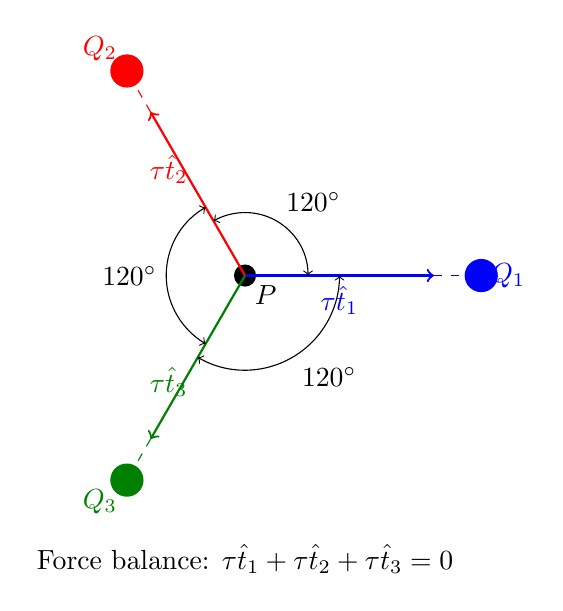
\begin{tikzpicture}[scale=2]
    % Junction point
    \coordinate (P) at (0,0);
    \fill (P) circle (2pt) node[below right] {$P$};

    % Three arms at 120 degrees
    \coordinate (Q1) at (0:1.5);
    \coordinate (Q2) at (120:1.5);
    \coordinate (Q3) at (240:1.5);

    % Draw arms with arrows
    \draw[->,thick,blue] (P) -- (0:1.2) node[midway,below] {$\tau\hat{t}_1$};
    \draw[->,thick,red] (P) -- (120:1.2) node[midway,above left] {$\tau\hat{t}_2$};
    \draw[->,thick,green!50!black] (P) -- (240:1.2) node[midway,below left] {$\tau\hat{t}_3$};

    % Quarks
    \fill[blue] (Q1) circle (3pt) node[right] {$Q_1$};
    \fill[red] (Q2) circle (3pt) node[above left] {$Q_2$};
    \fill[green!50!black] (Q3) circle (3pt) node[below left] {$Q_3$};

    % Dashed lines to quarks
    \draw[dashed,blue] (0:1.2) -- (Q1);
    \draw[dashed,red] (120:1.2) -- (Q2);
    \draw[dashed,green!50!black] (240:1.2) -- (Q3);

    % Angle arcs
    \draw[<->] (0:0.4) arc (0:120:0.4) node[midway,above right] {$120\degree$};
    \draw[<->] (120:0.5) arc (120:240:0.5) node[midway,left] {$120\degree$};
    \draw[<->] (240:0.6) arc (240:360:0.6) node[midway,below right] {$120\degree$};

    % Force balance annotation
    \node at (0,-1.8) {Force balance: $\tau\hat{t}_1 + \tau\hat{t}_2 + \tau\hat{t}_3 = 0$};
\end{tikzpicture}
\caption{Y-junction with equal tensions. The three unit vectors $\hat{t}_i$ sum to zero only when they are separated by $120\degree$ angles. This is the Steiner configuration.}
\label{fig:steiner}
\end{figure}

\begin{remark}[Historical note]
This result was known to Fermat (1637) for the ``Fermat point'' problem and proven rigorously by Steiner (1837). In EDC, we derive it from first principles as a consequence of energy minimization, not as an imported theorem.
\end{remark}

\begin{lemma}[Riemannian Generalization \textup{\tagDer}]
\label{lem:riemannian-steiner}
Let $(\mathcal{M}, g)$ be a Riemannian manifold and $\mathcal{N}$ a network of three geodesic arcs meeting at a junction point $P$. The first variation of the weighted length functional $L = \sum_i \tau_i \ell_i$ with respect to variations of $P$ gives:
\begin{equation}
\sum_{i=1}^{3} \tau_i \, \hat{t}_i = 0 \quad \text{in } T_P\mathcal{M}
\end{equation}
where $\hat{t}_i$ are unit tangent vectors at $P$ measured in the metric $g$.
\end{lemma}

\begin{proof}
In Riemannian geometry, geodesics locally minimize length. The variation of arc length under junction displacement $\delta P$ gives $\delta \ell_i = -g(\hat{t}_i, \delta P)$ to first order. Summing with weights $\tau_i$ and requiring stationarity for all $\delta P \in T_P\mathcal{M}$ yields the result.
\end{proof}

\begin{corollary}[120\degree{} in Local Metric \textup{\tagDer}]
For equal tensions $\tau_1 = \tau_2 = \tau_3$ in any Riemannian manifold, the equilibrium angles are $120\degree$ \emph{as measured in the local metric} at $P$. This is a universal geometric optimum, not specific to flat space or QCD.
\end{corollary}

\begin{remark}[Global positioning \textup{\tagOpen}]
While the \emph{local} angle condition is universal, the \emph{global} problem of finding the optimal junction position $P$ given fixed quark positions $\{Q_i\}$ depends on the full geometry of $(\Mfive, g)$. In curved bulk, geodesics may not be straight lines, and multiple local minima may exist. This global optimization remains an open problem for general 5D metrics.
\end{remark}

\subsection{Unequal Tension Case: Lami's Theorem}

\begin{theorem}[Generalized Angles \textup{\tagDer}]
\label{thm:lami}
For unequal tensions $\tau_1, \tau_2, \tau_3$, the equilibrium angles satisfy Lami's theorem:
\begin{equation}
\frac{\tau_1}{\sin\theta_{23}} = \frac{\tau_2}{\sin\theta_{31}} = \frac{\tau_3}{\sin\theta_{12}}
\end{equation}
where $\theta_{jk}$ is the angle between arms $j$ and $k$ (measured on the side not containing arm $i$).
\end{theorem}

\begin{proof}
From Eq.~\eqref{eq:force-balance}, the three tension vectors form a closed triangle. By the sine rule for triangles:
\begin{equation}
\frac{|\tau_1 \hat{t}_1|}{\sin(\pi - \theta_{23})} = \frac{|\tau_2 \hat{t}_2|}{\sin(\pi - \theta_{31})} = \frac{|\tau_3 \hat{t}_3|}{\sin(\pi - \theta_{12})}
\end{equation}
Since $\sin(\pi - x) = \sin x$ and $|\hat{t}_i| = 1$, this gives Lami's result.
\end{proof}

\begin{corollary}[Equal Tension Recovery]
Setting $\tau_1 = \tau_2 = \tau_3$ in Lami's theorem gives $\sin\theta_{12} = \sin\theta_{23} = \sin\theta_{31}$, hence all angles equal $120\degree$ (since they must sum to $360\degree$).
\end{corollary}

\begin{remark}[Qualitative prediction: flavor $\to$ angle deviations \textup{\tagP}/\textup{\tagOpen}]
\label{rem:flavor-prediction}
The Lami generalization provides a \textbf{conceptual prediction} for heavier baryons:
\begin{itemize}[nosep]
    \item If quark ``flavor'' (mass difference, coupling strength) translates to different effective arm tensions $\tau_i$, then equilibrium angles must deviate from $120\degree$.
    \item For baryons with one heavier quark (e.g., $\Lambda^0$ with $uds$), the heavier-flavor arm would have higher tension, pulling its neighbors closer.
    \item This qualitative discriminator could distinguish EDC predictions from symmetric-junction models.
\end{itemize}
\textbf{Status:} The mapping $\tau(\text{flavor})$ is not yet derived from EDC dynamics; this remains \tagOpen{}. However, the prediction is falsifiable: if heavier baryons show no angular asymmetry (via decay distributions or lattice QCD), the tension-flavor link is ruled out.
\end{remark}

% ------------------------------------------------------------
%  SUBSECTION 4.4: ACTION FORMULATION
% ------------------------------------------------------------
\subsection{Action-Level Formulation}
\label{subsec:action}

The variational analysis above can be derived from an explicit action principle. For a junction network of relativistic strings:

\begin{definition}[Junction Network Action \textup{\tagP}]
\label{def:junction-action}
The Nambu--Goto action for the junction network is:
\begin{equation}
S_{\text{junction}} = -\sum_{i=1}^{3} \tau_i \int d^2\xi \, \sqrt{-\det(\gamma_{i,ab})}
\label{eq:nambu-goto-action}
\end{equation}
where:
\begin{itemize}[nosep]
    \item $\tau_i$ is the tension of arm $i$ (energy per length, $[\tau] = E/L$)
    \item $\xi^a = (\xi^0, \xi^1)$ are worldsheet coordinates (time and spatial parameter)
    \item $\gamma_{i,ab} = g_{\mu\nu} \partial_a X_i^\mu \partial_b X_i^\nu$ is the induced metric on the $i$-th arm worldsheet
    \item $X_i^\mu(\xi)$ maps the worldsheet into the ambient 5D spacetime
\end{itemize}
\end{definition}

\begin{proposition}[Static Limit \textup{\tagDer}]
In the static limit (time-independent configurations), the action reduces to:
\begin{equation}
S = -T \cdot L[\mathcal{N}] = -T \sum_{i=1}^{3} \tau_i \ell_i
\end{equation}
where $T$ is the time duration and $\ell_i$ is the proper length of arm $i$. Minimizing $S$ is equivalent to minimizing the weighted length functional $L[\mathcal{N}]$.
\end{proposition}

\begin{remark}[Junction boundary term \textup{\tagOpen}]
The action Eq.~\eqref{eq:nambu-goto-action} implicitly requires a \textbf{junction boundary condition}: the three worldsheets share a common boundary curve (the junction worldline). The complete treatment requires a boundary action or constraint:
\begin{equation}
X_1^\mu(\xi^0, 0) = X_2^\mu(\xi^0, 0) = X_3^\mu(\xi^0, 0) = P^\mu(\xi^0)
\end{equation}
where $P^\mu(\xi^0)$ is the junction worldline. Variation with respect to $P^\mu$ yields the force balance condition $\sum_i \tau_i \hat{t}_i = 0$ as the junction equation of motion. A fully covariant treatment of this boundary condition (including the Gibbons--Hawking--York analogue for strings) remains \tagOpen{}.
\end{remark}

% ============================================================
%  SECTION 5: BRANE PROJECTION
% ============================================================
\section{Projection to 4D Brane}
\label{sec:projection}

\begin{proposition}[Angle Preservation under Projection \textup{\tagDc}]
\label{prop:projection}
If the junction vertex lies on the 4D brane $\Bfour$ and all three arm tangents $\hat{t}_i$ are tangent to $\Bfour$ at $P$, then the $120\degree$ angles are preserved in the brane-induced geometry.
\end{proposition}

\begin{proof}
The induced metric on $\Bfour$ restricts the 5D metric. If all tangent vectors lie in $T_P\Bfour$, then inner products (and hence angles) are computed with the same metric tensor. The force balance Eq.~\eqref{eq:force-balance} holds in the tangent space, which is the same whether viewed as part of $\Mfive$ or intrinsic to $\Bfour$.
\end{proof}

\begin{remark}[Bulk extension \textup{\tagOpen}]
If the arms extend into the 5D bulk away from the junction, their geometry is governed by the geodesic equation in $\Mfive$. The global minimization problem (finding the optimal junction position given quark positions) is more complex and may involve bulk curvature. This is left as an open problem for future work.
\end{remark}

\subsection{Frozen Projection Boundary (5D $\to$ 4D $\to$ 3D)}
\label{subsec:frozen-projection}

The transition from bulk (5D) description to brane-observed (3D) physics involves a \textbf{projection boundary condition} that determines which degrees of freedom remain dynamical and which become ``frozen.''

\begin{definition}[Frozen-Projection Boundary \textup{\tagP}]
\label{def:frozen-boundary}
Let $\pi: \Mfive \to \Bfour$ be the brane embedding and $\Pi: \Bfour \to \mathbb{R}^3$ the observational reduction (spatial projection). The \textbf{frozen boundary condition} acts on the composite map $\Pi \circ \pi$ as follows:

An internal degree of freedom with characteristic frequency $\omega$ is \textbf{frozen} when:
\begin{equation}
\hbar\omega \gg E_{\text{env}}
\label{eq:frozen-criterion}
\end{equation}
where $E_{\text{env}}$ is the relevant environmental energy scale (thermal $kT$, interaction energy, or probe resolution). Frozen DOFs are treated as fixed (Dirichlet/adiabatic constraint) in the effective 3D description.
\end{definition}

\begin{remark}[Two viewpoints on the proton \textup{\tagDc}]
\label{rem:two-viewpoints}
This framework distinguishes:
\begin{enumerate}[nosep]
    \item \textbf{Bulk-side (5D):} Each arm carries full state $\psi_i \in \text{SU}(2) \cong \Sthree$. The configuration space is $(\Sthree)^3$ with volume $(2\pi^2)^3$.
    \item \textbf{Brane/3D observed:} Only Hopf base variables $\hat{t}_i \in \Stwo$ are directly observable as spatial directions. The $S^1$ fiber phases are frozen by the boundary condition during projection.
\end{enumerate}
The mass calculation uses the \emph{bulk-side} volume $(2\pi^2)^3$ because mass is an intrinsic 5D property (energy stored in configuration), while observations access only the projected base.
\end{remark}

\begin{remark}[Connection to electron $\Bthree$ \textup{\tagDc}]
\label{rem:frozen-electron}
For the electron (simple vortex), the frozen condition is more severe: boundary terms at the $\xi$-scale freeze \emph{all} internal orientation DOFs to a ball $\Bthree$ rather than a sphere $\Sthree$. This explains why $C_e = \text{Vol}(\Bthree) = 4\pi/3$ rather than $\text{Vol}(\Sthree) = 2\pi^2$.

The proton's extended Y-junction structure allows more internal freedom (three SU(2) arms) that survives the frozen projection, yielding the factor $6\pi^5$ in the mass ratio.
\end{remark}

\begin{remark}[Mechanism status \textup{\tagOpen}]
The physical mechanism implementing Eq.~\eqref{eq:frozen-criterion} remains an open problem. Two candidate mechanisms merit investigation:
\begin{enumerate}[nosep]
    \item \textbf{Boundary-induced spectral gap} \tagOpen{}/\tagP{}: Dirichlet conditions at the brane boundary discretize the fiber modes, creating a gap $\Delta E \sim \hbar/R_\xi$. When $\Delta E \gg kT$, only the ground state is occupied---effectively ``freezing'' the fiber phase.
    \item \textbf{Observational coarse-graining} \tagOpen{}/\tagP{}: The 3D observer's measurement apparatus cannot resolve $S^1$ fiber phases below some scale. This is analogous to decoherence: fiber superpositions appear classical (fixed) when traced over unobserved environmental DOFs.
\end{enumerate}
What is established is the \emph{consequence}: bulk DOFs split into observable base ($\Stwo$) and frozen fiber ($S^1$). The mechanism determines \emph{which} DOFs freeze, but the geometric split is robust.
\end{remark}

\begin{figure}[h]
\centering
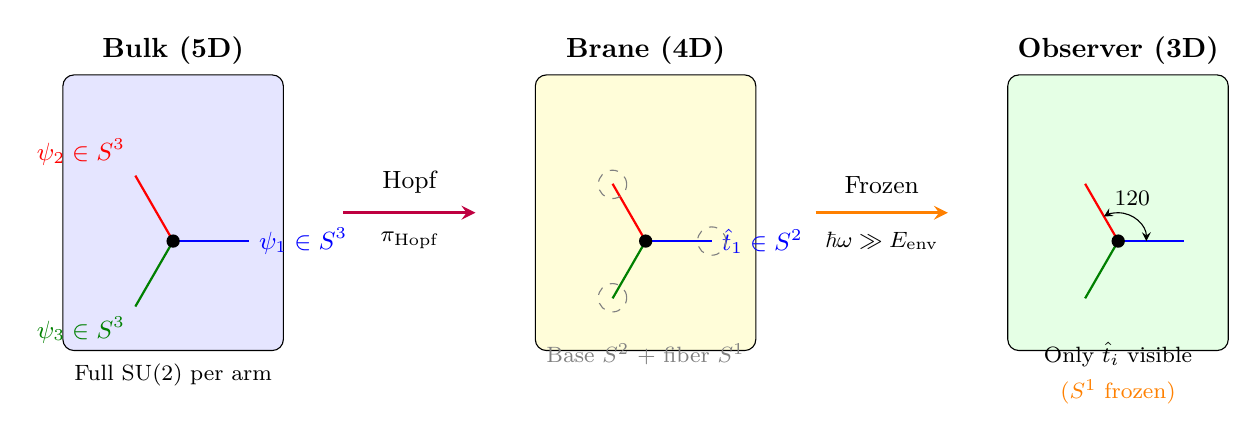
\begin{tikzpicture}[scale=1.2, >=stealth]
    % === LEFT: BULK (5D) ===
    \node[draw, rounded corners, fill=blue!10, minimum width=2.8cm, minimum height=3.5cm] (bulk) at (0,0) {};
    \node[above] at (bulk.north) {\textbf{Bulk (5D)}};

    % Three arms in bulk
    \coordinate (J) at (0,-0.3);
    \draw[thick, blue] (J) -- ++(0:0.8) node[right, font=\small] {$\psi_1 \in S^3$};
    \draw[thick, red] (J) -- ++(120:0.8) node[above left, font=\small] {$\psi_2 \in S^3$};
    \draw[thick, green!50!black] (J) -- ++(240:0.8) node[below left, font=\small] {$\psi_3 \in S^3$};
    \fill (J) circle (2pt);
    \node[below, font=\footnotesize] at (0,-1.5) {Full SU(2) per arm};

    % === ARROW 1: Hopf projection ===
    \draw[->, very thick, purple] (1.8,0) -- (3.2,0);
    \node[above, font=\small] at (2.5,0.1) {Hopf};
    \node[below, font=\footnotesize] at (2.5,-0.1) {$\pi_{\text{Hopf}}$};

    % === MIDDLE: BRANE (4D) with fiber ===
    \node[draw, rounded corners, fill=yellow!15, minimum width=2.8cm, minimum height=3.5cm] (brane) at (5,0) {};
    \node[above] at (brane.north) {\textbf{Brane (4D)}};

    % Base S² with fiber S¹
    \coordinate (J2) at (5,-0.3);
    \draw[thick, blue] (J2) -- ++(0:0.7) node[right, font=\small] {$\hat{t}_1 \in S^2$};
    \draw[thick, red] (J2) -- ++(120:0.7);
    \draw[thick, green!50!black] (J2) -- ++(240:0.7);
    \fill (J2) circle (2pt);

    % Fiber circles (dashed)
    \draw[dashed, gray] (5.7,-0.3) circle (0.15);
    \draw[dashed, gray] (4.65,0.3) circle (0.15);
    \draw[dashed, gray] (4.65,-0.9) circle (0.15);
    \node[font=\footnotesize, gray] at (5,-1.5) {Base $S^2$ + fiber $S^1$};

    % === ARROW 2: Frozen projection ===
    \draw[->, very thick, orange] (6.8,0) -- (8.2,0);
    \node[above, font=\small] at (7.5,0.1) {Frozen};
    \node[below, font=\footnotesize] at (7.5,-0.1) {$\hbar\omega \gg E_{\text{env}}$};

    % === RIGHT: OBSERVER (3D) ===
    \node[draw, rounded corners, fill=green!10, minimum width=2.8cm, minimum height=3.5cm] (obs) at (10,0) {};
    \node[above] at (obs.north) {\textbf{Observer (3D)}};

    % Only directions visible
    \coordinate (J3) at (10,-0.3);
    \draw[thick, blue] (J3) -- ++(0:0.7);
    \draw[thick, red] (J3) -- ++(120:0.7);
    \draw[thick, green!50!black] (J3) -- ++(240:0.7);
    \fill (J3) circle (2pt);

    % 120° label
    \draw[<->] (10,-0.3) ++(0:0.3) arc (0:120:0.3);
    \node[font=\footnotesize] at (10.15,0.15) {$120°$};

    \node[font=\footnotesize] at (10,-1.5) {Only $\hat{t}_i$ visible};
    \node[font=\footnotesize, orange] at (10,-1.9) {($S^1$ frozen)};
\end{tikzpicture}
\caption{Projection chain from 5D bulk to 3D observation. \textbf{Left:} In the bulk, each arm carries full SU(2) $\cong S^3$ orientation. \textbf{Middle:} Hopf fibration splits this into base $S^2$ (direction) and fiber $S^1$ (phase). \textbf{Right:} The 3D observer sees only the base directions $\hat{t}_i \in S^2$; fiber phases are frozen under criterion $\hbar\omega \gg E_{\text{env}}$. The $120\degree$ angles are preserved throughout.}
\label{fig:projection-chain}
\end{figure}

% ============================================================
%  SECTION 6: CONNECTION TO PAPER 2
% ============================================================
\section{Connection to Paper 2}
\label{sec:paper2}

\subsection{Configuration Space}

Paper 2 introduces the proton configuration space:
\begin{equation}
Q_{\text{proton}} = \Sthree \times \Sthree \times \Sthree
\end{equation}
where each $\Sthree$ factor represents the orientation degrees of freedom of one arm.

\begin{definition}[Physical Configuration Space \textup{\tagOpen}]
\label{def:qphys}
The \textbf{physical} (gauge-inequivalent) configuration space requires quotienting by:
\begin{enumerate}[nosep]
    \item Global rotations: SO(3) or SU(2) acting diagonally on all three arms
    \item Discrete relabeling: $\Zthree$ permutations of identical arms (for equal quark masses)
\end{enumerate}
Schematically:
\begin{equation}
Q_{\text{phys}} = \frac{(\Sthree)^3}{\text{SU}(2)_{\text{diag}} \times \Zthree}
\end{equation}
The precise quotient structure (whether to use SU(2), SO(3), or their subgroups) depends on boundary conditions and $\xi$-winding selection rules. \textbf{This remains an open problem} \tagOpen{}.
\end{definition}

\begin{remark}[Working Convention \textup{\tagDc}]
\label{rem:working-convention}
In this paper and Paper 2, we compute volumes using the \emph{un-quotiented} space $(\Sthree)^3$:
\begin{equation}
C_p = \text{Vol}((\Sthree)^3) = (2\pi^2)^3
\end{equation}
This serves as an upper bound or idealization.

\textbf{Gauge redundancy:} Modding out by diagonal SU(2) removes redundant global rotations. For a continuous gauge group, proper treatment requires gauge-fixing and Haar measure normalization (Faddeev--Popov procedure), not naive ``division by $|\text{SU}(2)|$'' \tagOpen{}. The discrete $\Zthree$ permutation contributes a finite factor of 3 (or 1 if arms are distinguishable by flavor).

\textbf{Cancellation caveat:} One might expect quotient factors to cancel in $m_p/m_e = C_p/C_e$. However, this cancellation is \emph{not guaranteed} because:
\begin{itemize}[nosep]
    \item Proton uses $(\Sthree)^3$ with SU(2)$_{\text{diag}}$ redundancy
    \item Electron uses $\Bthree$ (ball) with different frozen manifold
\end{itemize}
Consistent gauge-inequivalent measures for both particles remain \tagOpen{}. The \emph{relative} ratio $6\pi^5$ is expected to be robust at leading order; corrections are $O(1)$ at most.
\end{remark}

\subsection{The Hopf Bridge: $\Sthree \to \Stwo$ with $S^1$ Fiber}
\label{subsec:hopf}

The apparent mismatch between $\Sthree$ (Paper 2) and $\Stwo$ (junction plane tangents) is resolved by the \textbf{Hopf fibration}---a fundamental structure in topology and physics.

\begin{postulate}[Arm Internal Structure \textup{\tagP}]
\label{post:arm-internal}
Each flux-tube arm carries an \textbf{internal $S^1$ phase} (winding/orientation degree of freedom) in addition to its spatial direction. The total orientation space for one arm is:
\begin{equation}
\text{SU}(2) \cong \Sthree
\end{equation}
which fibers over the visible direction $\Stwo$ with $S^1$ fiber:
\begin{equation}
S^1 \hookrightarrow \Sthree \xrightarrow{\pi_{\text{Hopf}}} \Stwo
\end{equation}
Explicitly, the Hopf map sends $\psi \in \text{SU}(2)$ to a unit vector via:
\begin{equation}
\hat{t} = \psi \, \sigma_3 \, \psi^{-1} \in \Stwo \subset \mathbb{R}^3
\label{eq:hopf-explicit}
\end{equation}
where $\sigma_3 = \text{diag}(1,-1)$ is the third Pauli matrix. Two elements $\psi, \psi'$ project to the same $\hat{t}$ iff $\psi' = \psi \cdot e^{i\phi\sigma_3/2}$ for some phase $\phi$---this is the $S^1$ fiber.
\end{postulate}

\begin{remark}[Physical interpretation of the fiber]
The $S^1$ fiber has multiple physical interpretations, with different epistemic status:
\begin{itemize}[nosep]
    \item \textbf{Winding number} \tagDc{}: Phase accumulated around the compact $\xi$-dimension. This follows directly from the KK structure: $\xi \sim \xi + 2\pi R_\xi$ implies $S^1$ periodicity in the fiber.
    \item \textbf{Kaluza-Klein mode} \tagDc{}: Momentum in the fifth dimension. Standard KK reduction identifies $S^1$ fiber momentum with discrete charge quantum.
    \item \textbf{Color phase} \tagI{}: Internal SU(3) orientation of the flux tube. This is an \emph{interpretation} linking the geometric $S^1$ to QCD color; the dynamical connection remains to be derived.
\end{itemize}
The key point: from the 4D brane, we see only the $\Stwo$ projection (tangent direction), but the full 5D description requires $\Sthree$.
\end{remark}

\begin{theorem}[Configuration Space from Hopf Structure \textup{\tagDc}]
\label{thm:config-hopf}
Given Postulate~\ref{post:arm-internal}, the proton configuration space is:
\begin{equation}
Q_{\text{proton}} = \text{SU}(2)^3 \cong \Sthree \times \Sthree \times \Sthree
\end{equation}
with volume:
\begin{equation}
\boxed{C_p = \text{Vol}(Q_{\text{proton}}) = \left( 2\pi^2 \right)^3}
\end{equation}
This is \tagDc{} (deduced from the arm internal structure postulate), \emph{not} numerology.
\end{theorem}

\begin{proof}
Each arm carries SU(2) $\cong \Sthree$ orientation. Three independent arms give $(\Sthree)^3$. The volume of $\Sthree$ is $2\pi^2$ (standard result). Thus $\text{Vol}(Q) = (2\pi^2)^3$.
\end{proof}

\begin{remark}[$C_e$ vs $\text{Vol}(\Sthree)$: Different objects \textup{\tagDc}]
\label{rem:ce-vs-s3}
A potential source of confusion:
\begin{itemize}[nosep]
    \item \textbf{Proton arm:} Configuration space is $\Sthree \cong \text{SU}(2)$, with $\text{Vol}(\Sthree) = 2\pi^2$
    \item \textbf{Electron:} Configuration space is $\Bthree$ (the 3-ball), with $\text{Vol}(\Bthree) = \frac{4\pi}{3}$
\end{itemize}
These are \emph{different topological objects}: $\Sthree$ is a 3-sphere (boundary of 4-ball), while $\Bthree$ is a 3-ball (solid ball in 3D). The electron is a ``frozen'' vortex defect whose orientation is constrained to a ball (see Companion E, Frozen Criterion), while each proton arm is an extended flux tube with full SU(2) internal structure.

The mass ratio formula uses:
\begin{equation}
\frac{m_p}{m_e} = \frac{C_p}{C_e} = \frac{(2\pi^2)^3}{4\pi/3} = 6\pi^5
\end{equation}
where $C_p = \text{Vol}((\Sthree)^3)$ and $C_e = \text{Vol}(\Bthree)$.
\end{remark}

\begin{remark}[Why this resolves the dimension mismatch]
\begin{itemize}[nosep]
    \item \textbf{Junction plane tangents:} $\hat{t}_i \in \Stwo$ (what force-balance sees)
    \item \textbf{Full arm state:} $\psi_i \in \Sthree$ (includes internal phase)
    \item \textbf{Hopf projection:} $\pi_{\text{Hopf}}(\psi_i) = \hat{t}_i$
\end{itemize}
Force-balance constrains only the Hopf base variables ($\hat{t}_i \in \Stwo$); the fiber phases remain dynamically free. However, the configuration-space volume $C_p$ is computed with the standard Haar measure on SU(2) for each arm, so no extra multiplicative $(2\pi)$ factors are introduced beyond $\text{Vol}(S^3) = 2\pi^2$.
\end{remark}

\subsection{Junction Constraint on the Base}

\begin{proposition}[Constraint Manifold \textup{\tagDc}]
The force balance condition (Eq.~\ref{eq:force-balance}) with equal tensions defines a constraint on the \emph{base} of the Hopf fibration:
\begin{equation}
\Sigma_{\text{base}} = \left\{ (\hat{t}_1, \hat{t}_2, \hat{t}_3) \in \Stwo \times \Stwo \times \Stwo \;\middle|\; \hat{t}_1 + \hat{t}_2 + \hat{t}_3 = 0 \right\}
\end{equation}
The full configuration space is the $S^1 \times S^1 \times S^1$ fibration over $\Sigma_{\text{base}}$.
\end{proposition}

\begin{remark}[Dimension accounting \textup{\tagDc}]
\begin{align}
\dim(\Stwo \times \Stwo \times \Stwo) &= 6 \\
\text{Constraints: } \sum \hat{t}_i = 0 &\to -2 \\
\dim(\Sigma_{\text{base}}) &= 4 \\
\text{Fiber: } S^1 \times S^1 \times S^1 &\to +3 \\
\dim(\text{total}) &= 7
\end{align}
After quotienting by overall rotation (global SO(3) or SU(2)), the effective dimension matches the expected proton internal degrees of freedom.

\textbf{Remaining open question} \tagOpen{}: Precise identification of which fiber combinations are physical (vs gauge redundancy) requires a detailed treatment of the $\xi$-winding boundary conditions.
\end{remark}

% ============================================================
%  SECTION 7: SUMMARY
% ============================================================
\section{Summary and Epistemic Classification}

\subsection{Main Results}

\begin{enumerate}
    \item \textbf{Force Balance} (Theorem \ref{thm:force-balance}): $\sum_i \tau_i \hat{t}_i = 0$ at equilibrium \tagDer{}

    \item \textbf{120\degree{} Angles} (Theorem \ref{thm:steiner}): Equal tensions imply Steiner configuration \tagDer{}

    \item \textbf{Lami Generalization} (Theorem \ref{thm:lami}): Unequal tensions give angle formula \tagDer{}

    \item \textbf{Brane Projection} (Proposition \ref{prop:projection}): Angles preserved on brane \tagDc{}
\end{enumerate}

\subsection{Epistemic Classification Table}

\begin{center}
\begin{tabular}{p{4cm}cc p{5cm}}
\toprule
\textbf{Claim} & \textbf{Tag} & \textbf{Ref} & \textbf{Notes} \\
\midrule
Baryon = 3-arm junction & \tagP{} & Post.~\ref{post:junction} & Foundational hypothesis \\
Brane embedding & \tagP{} & Post.~\ref{post:brane} & Junction on 4D brane \\
Equilibrium = min length & \tagP{} & Post.~\ref{post:equilibrium} & Nambu--Goto thin-string limit \\
Arm internal $S^1$ phase & \tagP{} & Post.~\ref{post:arm-internal} & Hopf fiber interpretation \\
\midrule
Force balance $\sum \tau_i \hat{t}_i = 0$ & \tagDer{} & Thm.~\ref{thm:force-balance} & Explicit variational proof \\
Equal tension $\Rightarrow 120\degree$ & \tagDer{} & Thm.~\ref{thm:steiner} & Explicit calculation \\
Lami's theorem & \tagDer{} & Thm.~\ref{thm:lami} & Sine rule application \\
\midrule
Angle preservation & \tagDc{} & Prop.~\ref{prop:projection} & Follows from tangent constraint \\
$C_p = (2\pi^2)^3$ & \tagDc{} & Thm.~\ref{thm:config-hopf} & From SU(2)$^3$ via Hopf bridge \\
$\Sthree \to \Stwo$ resolution & \tagDc{} & \S\ref{subsec:hopf} & Hopf fibration with $S^1$ fiber \\
\midrule
Bulk geodesics & \tagOpen{} & Rem.~5.1 & Global minimization in 5D \\
Fiber gauge redundancy & \tagOpen{} & Rem.~6.4 & Which fiber combos are physical \\
\bottomrule
\end{tabular}
\end{center}

\subsection{Calibration Boundary}

\textbf{This companion has zero calibrated parameters.}

The tension $\tau$ enters as an overall scale but cancels in all angle calculations. The $120\degree$ result is purely geometric, following from the postulate that baryons minimize weighted network length.

% ============================================================
%  SECTION 8: CONCLUSION
% ============================================================
\section{Conclusion}

We have derived the $120\degree$ Y-junction geometry from variational principles, providing the foundational support for Paper 2's proton model. The key insight is that the Steiner configuration is not an external input but a \emph{consequence} of energy minimization for equal-tension flux tubes.

\textbf{What this companion establishes:}
\begin{itemize}
    \item The $120\degree$ angles are \tagDer{}, not merely cited
    \item The derivation requires only the junction postulate \tagP{}
    \item The geometry projects naturally to the 4D brane \tagDc{}
    \item The $\Sthree$ vs $\Stwo$ mismatch is resolved via Hopf fibration \tagDc{}
    \item $C_p = (2\pi^2)^3$ follows from SU(2)$^3$ arm structure \tagDc{}
\end{itemize}

\textbf{What remains open:}
\begin{itemize}
    \item WHY baryons are junctions (vs other topologies) --- this is \tagP{}
    \item Global minimization in curved 5D bulk --- \tagOpen{}
    \item Precise identification of physical vs gauge-redundant fiber combinations --- \tagOpen{}
\end{itemize}

\subsection*{Cornerstone Statement}

\begin{tcolorbox}[colback=blue!5,colframe=blue!40!black,title=\textbf{Proton Geometry: The Variational Foundation}]
\textbf{Given} the junction postulate (baryons = 3-arm flux-tube networks in 5D):
\begin{enumerate}[nosep]
    \item The Steiner $120\degree$ configuration is \tagDer{} from energy minimization
    \item The configuration space $Q = \Sthree \times \Sthree \times \Sthree$ is \tagDc{} from the Hopf bridge
    \item The proton form factor $C_p = (2\pi^2)^3$ is \tagDc{}, not numerology
\end{enumerate}
\textbf{This is the geometric foundation for the proton in 5D EDC.}

All subsequent proton physics (Companion G: mass difference, Paper 2: mass ratio) inherits this variational foundation.
\end{tcolorbox}

\vspace{1em}
Companion G builds on this foundation to derive the neutron-proton mass difference from $\Zsix$ symmetry breaking.

\vspace{2em}
\hrule
\vspace{1em}
\noindent\textit{Companion F to Paper 3: NJSR Edition}\\
\textit{Completed: \today}

\end{document}
